\documentclass[times, 10pt,twocolumn]{article} 
\usepackage{latex8}
\usepackage{times}
\usepackage{amsmath}
\usepackage{amsthm}
\usepackage{graphicx}
\usepackage{url}
\usepackage[utf8x]{inputenc}
\usepackage[T1]{fontenc}
\usepackage{color}


\newtheorem{theorem}{Theorem}[section]

\newcommand{\comentario}[1]{}
\newcommand{\superscript}[1]{\ensuremath{^{\textrm{#1}}}}
\newcounter{notecounter}
\newcommand{\nota}[1]{\addtocounter{notecounter}{1}{\textcolor{red}{[nota
      \arabic{notecounter}: #1]}}}

\newcommand{\gnota}[1]{
  \addtocounter{notecounter}{1}
  \vspace{.5cm}
  \framebox{
    \begin{minipage}{0.95\linewidth}
      \textbf{nota \arabic{notecounter}:} #1
    \end{minipage}
  }\vspace{.5cm}}

\newcommand{\simul}{\textbf{Simul}} % Que criatividade. Mudar esse
% nome depois, urgente

\author{George Lima, Alexandre Passos, José Augusto Matos Santos}
\title{Hard Reservation vs Soft Reservation for soft real-time systems}

\begin{document}
\maketitle

\begin{abstract}

  When scheduling soft real-time tasks it is usually a good idea to
  reserve fractions of the total bandwidth to each task (or task
  group). This reservation might be either \textbf{hard}, when under
  no circumstances a task might use some extra bandwidth, or
  \textbf{soft}, if there are some situations when it is allowed to do
  so. Usually, specially in the context of on-line adaptative systems,
  hard reservation is perceived to be more predictable, stricter and
  allowing faster adaptation. In this paper we argue that, perhaps
  surprisingly, allowing tasks to use some idle bandwidth shouldn't
  hurt. To clarify our arguments we present the results of a few
  experiments performed on real-life and syntetic data sets using hard
  and soft variations of CBS, a commonly used reservation-based
  server.
  
\end{abstract}

\section{Introduction}
\label{sec:introduction}

In reservation-based scheduling of soft real-time tasks, each task is
allowed at most a given fraction of the total processor time. There
are two broad approaches to using said fraction: \textbf{hard} and
\textbf{soft} reservation. In a hard reservation framework each server
is allowed a given fraction of the total processing time, and in no
ocasion can use more than that fraction. If in some circumstances, a
pending task that has overrun its budget is allowed to use idle
processing time, then the reservation is said to be soft\nota{colocar
  referência da definição}. It is commonly acknowledged that a system
based on hard reservation is more predictable, if not more efficient,
than a system based on soft reservation. In this paper we present a
simulation environment for becnhmarking both reservation mechanisms
and experimental results in this environment that fail to show any
significant benefit either in predictability or in performance.

\subsection{Related work}
\label{sec:related-work}

In a paper on QoS management thourgh adaptive reservations
\cite{abeni.ea05:qos}, Abeni et al use a hard reservation approach to
help adaptivity. The need for such a restriction on the reservation
will be studied \nota{colocar um experimento com hard e soft
  corretamente dimensionados e variância maior/menor pra ver o que
  acontece} later in this paper.

\subsection{Contributions of this paper}
\label{sec:contr-this-paper}

The main contribution of this paper is putting into perspective the
perceived characteristics of hard reservation. There is a lack in
literature of experiments in a fair environment that measure
objectively the possible benefits and costs of using hard and soft
reservation in a given system.

\gnota{
    
É interessante discutir o teorema de butazzo do livro, pag 122

\begin{theorem}
  Given a CBS server with the hard reservation rule, and with
  parameters $(Q,P)$, if $k =
  \left\lceil\frac{t-(P-Q)}{P}\right\rceil$, the partition with the
  maximum delay that it can generate has the following least supply
  function $S^*(t)$:
  \[ S^*(t) = \left\{ \begin{array}{ll}
      0 & \text{if}\ t \in [0,P-Q] \\
      (k-1)Q & \text{if}\ t \in (kP - Q, (k+1)P-2Q) \\
      t-(k+1)(P-Q) & \text{otherwise.}
    \end{array}\right.
  \]
\end{theorem}

Esse teorema é usado pra dar limites no delay de um servidor.

Isso é usado no teorema

\begin{theorem}
  Let $A$ be set of periodic or sporadic tasks
  $\{\tau_1,\ldots,\tau_n\}$, with $\tau_i = (C_i,T_i,D_i)$, where
  $C_i$ is the worst-case computation time, $T_i$ is the task period
  and $D_i$ is the relative deadline. This task set is schedulable by
  EDF scheduling algorithm on a resource partition with least supply
  function $S^*(t)$ if and only if:
  \[
  \forall 0 < t \leq 2H : dbf(t) \leq S^*(t)
  \]
  where $H = lcm(T_1,\ldots,T_n)$ is the hyperperiod of A and $dbf(t)$
  is the processor demand bound function, defined as
  \[
  dbf(t) = \sum_{i=1}^n
  \left(\left\lfloor\frac{t-D_i}{T_i}\right\rfloor + 1\right)C_i.
  \]
\end{theorem}

Depois disso butazzo prova a fórmula de york para o tempo de
resposta. O primeiro desses teoremas é provado, o segundo não
exatamente, mas paciência.
}

\comentario{ 


medir número de preempções, é complicado, mas com simpy novo deve dar


Grande quantidade de trabalhos relativos ao uso de reservação de
banda. Falta de estudos comparativos sobre hard/soft. Conexão com
aplicações que poderiam se beneficiar do estudo.


}

\section{Simulation environment}
\label{sec:simul-envir}

To perform the experiments presented in this paper we implemented
\simul{}, a simple python-based simulator for real-time scheduling
algorithms. Its source code, the data files used in this paper and
instructions to reproduce our results are available in
\url{http://github.com/jamsjr/hard-versus-soft/tree/master}. \simul{}
implements a basic EDF scheduler and, on top of it, runs both hard
real-time periodic tasks and bandwidth sharing servers. These servers
can be either traditional CBS servers \nota{colocar referência para
  CBS} or a hard reservation adaptation of the CBS algorithm. Soft
real-time tasks running on these servers either have their execution
times sampled from a probability distribution or follow traces
generated from a modified version of mplayer\nota{citar mplayer?} that
reports the start time and decoding cost for each frame in a
high-definition video running on a XXX\nota{pegar info do pc de
  eduardo}.

\subsection{Controled variables}
\label{sec:controled-variables}

In our simulations we studied the possible effects of the given
variables:
\begin{itemize}
\item the \textbf{reservation style} can be either soft or hard, it's out
  objective to study the differences between these two;
\item \textbf{expired tasks} (tasks that ran over their deadlines)
  might be discarded or not;
\item the \textbf{execution costs} can be either from a real-life
  trace from a movie (shown in figure \ref{fig:plot-trace-eve}) or
  synthetic and normally distributed (seen in figure
  \ref{fig:plot-trace-normal});
\item when the execution costs are synthetic, their \textbf{variance}
  determines how much they stray from their expected value;
\item there might be \textbf{system idle time} or there might not;
\item the \textbf{server load} might be too high---meaning not all
  tasks can finish in the expected time---, correct---meaning all
  tasks should finish in the expected time---, or too low---meaning
  there will be substation idle time in the server.
\end{itemize}

\begin{figure}[t]
  \centering
  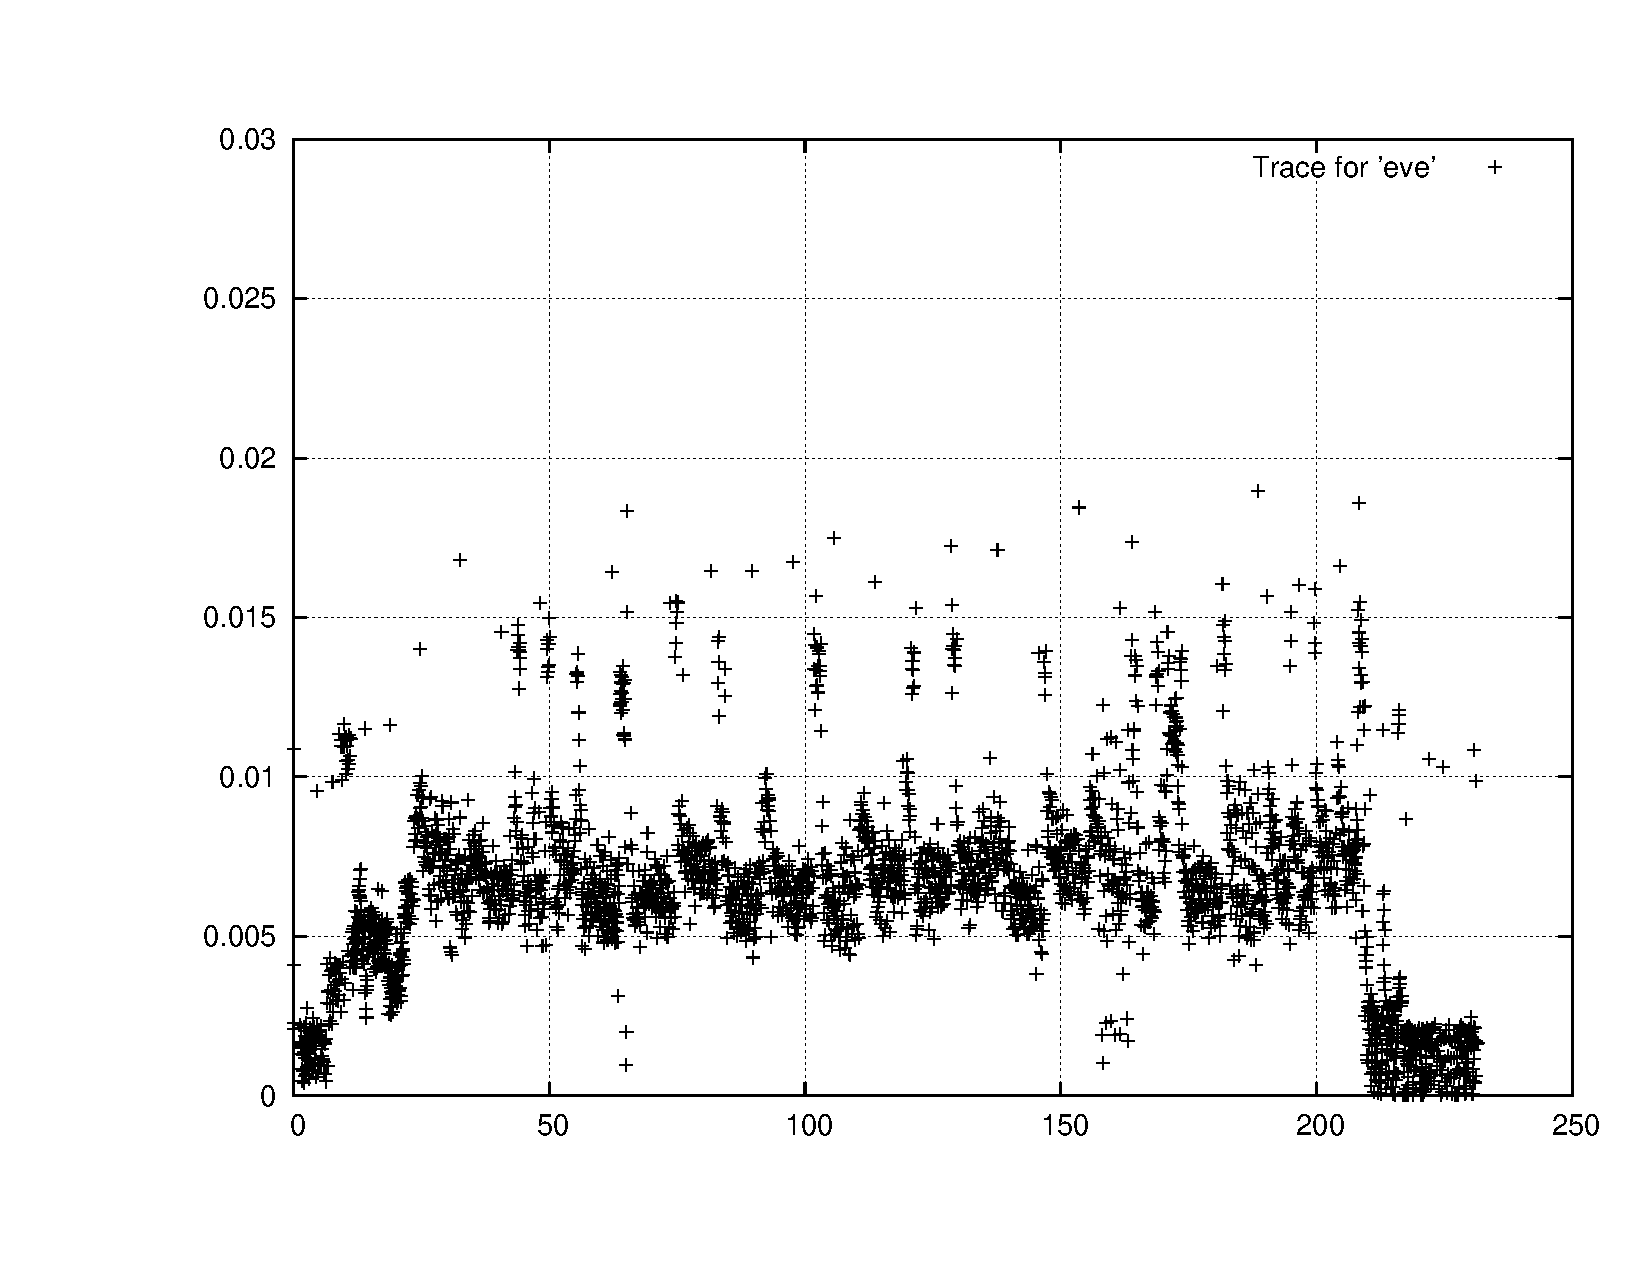
\includegraphics[scale=0.3]{trace-eve}
  \caption{Execution costs over time for the trace of the movie 'eve'.}
  \label{fig:plot-trace-eve}
\end{figure}

\begin{figure}[t]
  \centering
  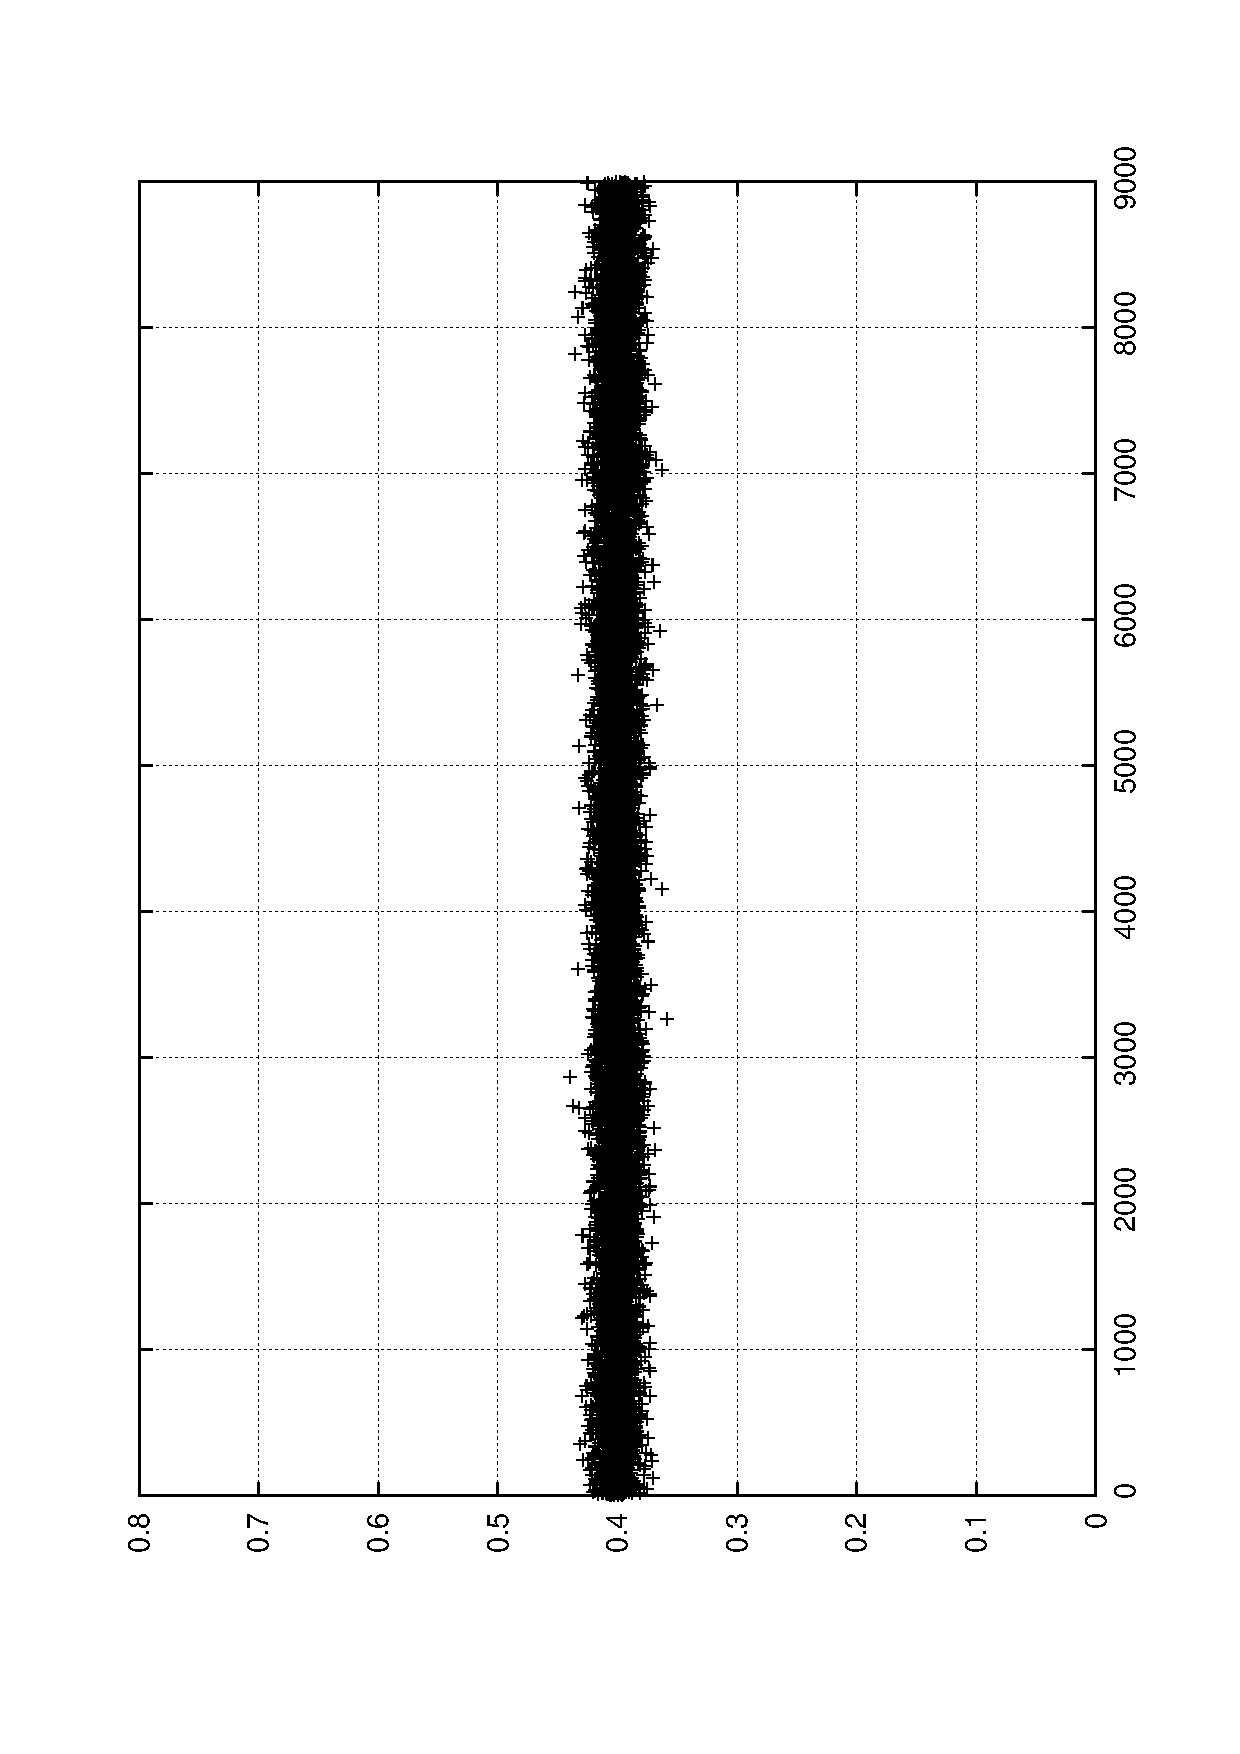
\includegraphics[scale=0.3]{trace-normal}
  \caption{Normally distributed execution costs over time.}
  \label{fig:plot-trace-normal}
\end{figure}

\comentario{
* Simulação
  
  Descrição do ambiente, modelo de tarefas, dados de entrada, etc.
}


\section{Performance Metrics}
\label{sec:metrics}

\comentario{   
* Métricas comparativas
  
  Descrição e conexão com aplicações.

  
** Tempo de resposta
   
   
** Intervalo entre deadlines
}


\section{Simulation Results}
\label{sec:simulation-results}

As can be seen in figures \nota{colocar as figuras}, soft reservation
usually outperforms hard reservation, having a smaller average
response time as well as a smaller worst-case response time, a shorter
delay between task arrival and start of execution, and a more uniform
interval between successive task terminations. Aside from the obvious
capacity of using extra free-time in a soft reservation framework,
some counter-intuitive 

\section{Conclusion}
\label{sec:conclusion}



\bibliographystyle{plain}
\bibliography{bib}
\end{document}
